\documentclass{article}
\usepackage{polski}
\usepackage[utf8]{inputenc}
\usepackage{amsmath}
\usepackage{amsfonts}
\usepackage{amssymb}
\usepackage{mathtools}
\usepackage{multirow}
\usepackage[table,xcdraw]{xcolor}
\usepackage{graphicx}
\usepackage{float}
\usepackage{placeins}
\usepackage[left=2cm,right=2cm,top=2.5cm,bottom=2.5cm]{geometry}

\makeatletter
\newcommand{\mathleft}{\@fleqntrue\@mathmargin0pt}
\newcommand{\mathcenter}{\@fleqnfalse}
\makeatother


\graphicspath{{Grafiki/}}

\title{Inteligentne systemy robotyczne\\Projekt\\Zima 2017/2018}
\author{Arkadiusz Piórkowski}

\begin{document}
%\pagenumbering{gobble}
\maketitle

%%%%%%%%%%%%%%%%%%%%%%%%%%%%%%%%%%%%%%%%%%%%%%%%%%%%%%%%%%%%%%%%%%%%%%%%%%%

\section*{Zadanie}

\begin{center}
\textit{Zadanie wybierania czerwonych sze\'scianów}
\end{center}

Należy zaprojektować system sterowania manipulatorem o sze\'sciu stopniach swobody wyposażonym w chwytak dwupalczasty z otwarciem sterowanym w sposób ciągly. Zadaniem robota jest wrzucanie czerwonych sze\'scianów poruszających się na ta\'smociągu do pojemnika. Nad ta\'smociągiem umieszczona jest typowa kamera RGB wchodząca w skład systemu. Na ta\'smociągu poruszają się sze\'sciany o różnych rozmiarach i kolorach. Szybko\'sć ruchu ta\'smociągu nie jest stała - ta\'smociąg nie jest sterowany przez projektowany system. Jego prędko\'sć mie\'sci się w zakresie $0.05~-~0.1~\mbox{m/s}$.

Stosując formalizm przedstawiony na wykładzie należy:
\begin{itemize}
\item Okre\'slić strukturę systemu w kategoriach agentów,
\item Dla każdego agenta należy zdefiniować podsystem sterowania, efektory i receptory wirutualne,
\item Dla tych podsystemów okre\'slić:
\begin{itemize}
\item Automat skończony sterujący ich pracą,
\item Zachowania,
\item Warunki początkowe i końcowe zachowań,
\item Funkcje przej\'scia (w postaci matematycznej i DFD),
\item Zawarto\'sć pamięci wewnętrznej oraz buforów wej\'sciowych i wyj\'sciowych,
\item Krok dyskretyzacji czasu dla każdego podsystemu.
\end{itemize}
\end{itemize}

%%%%%%%%%%%%%%%%%%%%%%%%%%%%%%%%%%%%%%%%%%%%%%%%%%%%%%%%%%%%%%%%%%%%%%%%%%%
\newpage

\tableofcontents
\pagebreak
%%%%%%%%%%%%%%%%%%%%%%%%%%%%%%%%%%%%%%%%%%%%%%%%%%%%%%%%%%%%%%%%%%%%%%%%%%%

\section{Założenia}

Podczas projektowania systemu sterowania przyjęto następujące założenia
\begin{itemize}
\item W obszarze widzianym przez kamerę możne znajdować się maksymalnie jeden sze\'scian,
\item Obszar ta\'smociągu widziany przez kamerę jest osiągalny przez manipulator,
\item Manipulator (efektor) nie powoduje zasłonięcia sze\'scianu podczas jego pobierania,
\item Pozycja pojemnika, kamery, ta\'smociągu oraz podstawy manipulatora są znane (położenie układów współrzędnych związanych z elementami systemu),
\item Chwytak pod wpływem zamknięcia (z okre\'slonym marginesem)  nie generuje niszczącej siły względem elementu pobieranego,
\item Otwarcie chwytaka sterowanego w sposób ciągły jest podawane w jednostkach długo\'sci, które są tłumaczone na odpowiednią warto\'sć sterującą przez regulatory rzeczywistego efektora,
\item Maksymalna prędko\'sć końcówki manipulatora wynosi 1 m/s.
\end{itemize}
\pagebreak


%%%%%%%%%%%%%%%%%%%%%%%%%%%%%%%%%%%%%%%%%%%%%%%%%%%%%%%%%%%%%%%%%%%%%%%%%%%

\section{Struktura systemu}

Projektowany system składa się z pojedynczego agenta $\hat{a} = \{a_1\}$. Na rysunku \ref{fig::struktura} przedstawiono przyjętą strukturę systemu.
\begin{figure}[H]
	\centering
	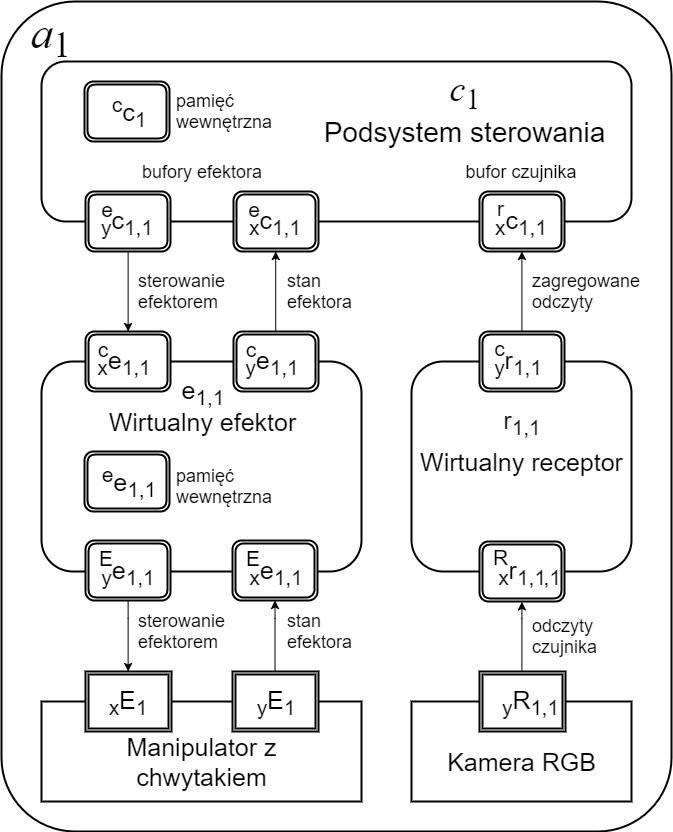
\includegraphics[width=0.8\textwidth]{struktura1.png}
	\caption{Struktura systemu sterowania}
	\label{fig::struktura}
\end{figure}
\noindent Upostaciowiony agent  $a_1$  składa się z następujących podsystemów:
\begin{itemize}
\item \textbf{Wirtualny receptor $\bold{r_{1,1}}$} - interfejs między układem sterowania, a \textbf{rzeczywistym efektorem}($E_1$) będącym manipulatorem o sze\'sciu stopniach swobody wyposażonym w chwytak dwupalczasty z otwarciem sterowanym w sposób ciągły. Wirtualny efektor upraszcza polecenia oraz informację przepływające między manipulatorem a podsystemem sterowania.
\item \textbf{Wirtualny efektor $\bold{e_{1,1}}$} - interfejs między układem sterowania, a \textbf{rzeczywistym receptorem}($R_1$) będącym typową kamerą RGB umieszczoną nad ta\'smociągiem. Wirtualny receptor jest odpowiedzialny za agregacje informacji przyłąnących z kamery(rzeczywisty receptor) i przesłanie ich do posystemu sterowania w celu wyznaczenia kolejnych kroków algorytmu.
\item \textbf{Podsystem sterowania $\bold{c_{1}}$} - odpowiedzialny komunikację z efektorem oraz czujnikiem i podejmujący decyzję o kolejnych krokach algorytmu.
\end{itemize}

%%%%%%%%%%%%%%%%%%%%%%%%%%%%%%%%%%%%%%%%%%%%%%%%%%%%%%%%%%%%%%%%%%%%%%%%%%%

\subsection{Podsystem sterowania}

\begin{figure}[H]
	\centering
	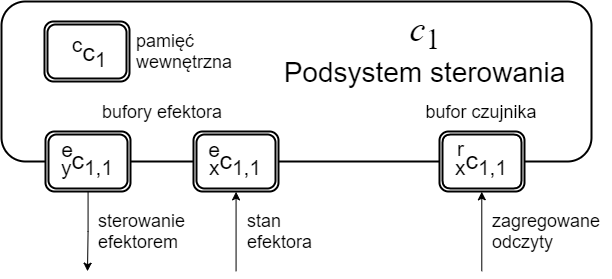
\includegraphics[width=0.85\textwidth]{podsystem_sterowania.png}
	\caption{Podsystem sterowania}
	\label{fig::podsystem_sterowania}
\end{figure}

\subsubsection{Zawarto\'sć pamięci wewnętrznej oraz buforów wej\'sciowych i wyj\'sciowych}
\begin{enumerate}
\item Pamięć wewnętrzna podsystemu sterowania:
\begin{itemize}
\item $^cc_{1}$ [$^0_PT,^0_CT, ^E_GT_d, ^E_PT_d, k, w_{max},w_p, n_d, STATUS$] - pozycja pojemnika względem układu globalnego, pozycja kamery względem układu globalnego, pożądana pozycja obiektu względem końcówki (chwytaka), pożądana pozycja pojemnika względem końcówki (chwytaka), margines zamknięcia chwytaka, maksymalne rozwarcie chwytaka, poprzednie rozwarcie chwytaka, pożądana liczba kroków efektora równa ilorazowi kroku dyskretyzacji czasu podsystemu sterowania i kroku dyskretyzacji czasu wirtualnego efektora, status podsystemu przyjmuje warto\'sci ``FREE''(pobieranie obiektu lub bezczynno\'sć) lub ``BUSY''(odkładanie pobranego obiektu do pojemnika).
\end{itemize}
\item Bufor z wirtualnego receptora:
\begin{itemize}
\item $^r_xc_{1,1}$ [$^C_GT_c, w$] - aktualna pozycja rozpoznawanego obiektu(czerwonego sze\'scianu) względem kamery, szeroko\'sć obiektu.
\end{itemize}
\item Bufor z wirtualnego efektora:
\begin{itemize}
\item $^e_xc_{1,1}$ [$^0_ET_c$] - aktualna kartezjańska pozycja bezwzględna.
\end{itemize}
\item Bufor do wirtualnego efektora:
\begin{itemize}
\item $^e_yc_{1,1}$ [$^ET_{d',c}, n_d, w_e$] - względna kartezjańska pozycja pożądana oraz liczba kroków, w których efektor ma ją osiągnąć, rozwarcie chwytaka.
\end{itemize}
\end{enumerate}

%------------------------------------------------------------------------------------------------------------------------------------------------------------------------------------------------------------

\subsubsection{Automat skończony, zachowania, warunki początkowe i końcowe}
\begin{figure}[H]
	\centering
	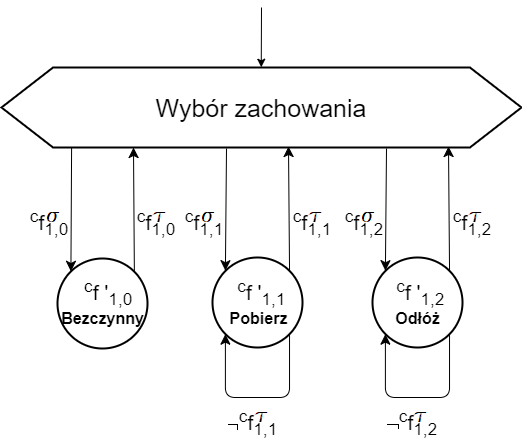
\includegraphics[width=0.55\textwidth]{PS_automat.png}
	\caption{Automat skończony zachowań podsystemu sterowania}
	\label{fig::PS_automat}
\end{figure}

Podsystem sterowania ma okre\'slone trzy zachowania: \textit{``Bezczynny''}, \textit{``Pobierz''} oraz \textit{``Odłóż''}. 
\newline
\begin{itemize}
\item Warunki początkowe i końcowe dla zachowania \textit{``Bezczynny''}:
\[^c_+B_{1,0}( ^{c}f'_{1,0}, ^cf^\tau_{1,0} )\]
\[^cf^\sigma_{1,0} \triangleq (\neg \mbox{new}(^r_xc_{1,1}) \wedge \mbox{STATUS} == \mbox{FREE}) = (\neg \mbox{new}(^C_GT_c,w) \wedge \mbox{STATUS} == \mbox{FREE}) \]
\[^cf^\tau_{1,0} \triangleq \mbox {True}\] 
Generator następnego stanu wirtualnego efektora:
\[ _yc^{i+1}_{1,1} = ^{c}f'_{1,0}(_xc^i_{1,1})\]

\item Warunki początkowe i końcowe dla zachowania \textit{``Pobierz''}:
\[^c_+B_{1,1}( ^{c}f'_{1,1}, ^cf^\tau_{1,1} )\]
\[^cf^\sigma_{1,1} \triangleq (\mbox{new}(^r_xc_{1,1}) \wedge \mbox{STATUS} == \mbox{FREE}) = (\mbox{new}(^C_GT_c,w) \wedge \mbox{STATUS} == \mbox{FREE}) \]
\[^cf^\tau_{1,1} \triangleq (\mbox{STATUS} == \mbox{BUSY})\]
Generator następnego stanu wirtualnego efektora:
\[ _yc^{i+1}_{1,1} = ^{c}f'_{1,1}(_xc^i_{1,1})\]

\item Warunki początkowe i końcowe dla zachowania \textit{``Odłóż'}:
\[^c_+B_{1,2}( ^{c}f'_{1,2}, ^ef^\tau_{1,2} )\]
\[^cf^\sigma_{1,2} \triangleq  (\mbox{STATUS} == \mbox{BUSY}) = ^cf^\tau_{1,1}\]
\[^cf^\tau_{1,2} \triangleq (\mbox{STATUS} == \mbox{FREE})\]
Generator następnego stanu wirtualnego efektora:
\[ _yc^{i+1}_{1,1} = ^{c}f'_{1,2}(_xc^i_{1,1})\]
\end{itemize}


%------------------------------------------------------------------------------------------------------------------------------------------------------------------------------------------------------------

\subsubsection{Funkcje przej\'scia}
\begin{itemize}

\item Funkcje przej\'scia dla zachowania \textit{``Bezczynny''}:
\begin{itemize}
\item Funkcja przej\'scia między podsystemem sterowania a efektorem wirtualnym (brak zmiany położenia efektora - wczytanie danych z pamięci wewnętrznej):
\[ ^e_yc_{1,1}^{i+1} \triangleq ^{c,e}f'_{1,0}(^cc_1^i) =
\begin{cases}
^ET_{d',c} = 0 \\
 n_d = n_d \\
w_e = w_p
\end{cases}\]
\begin{figure}[H]
	\centering
	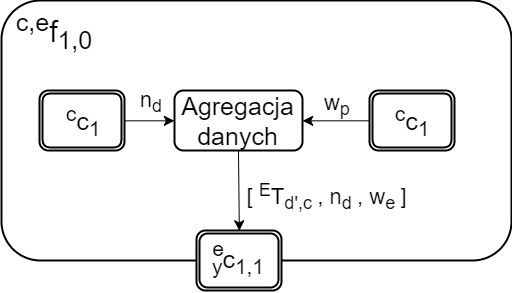
\includegraphics[width=0.4\textwidth]{PS_funkcje1v0.png}
	\caption{Funkcja przej\'scia podsystemu sterowania $^{c,e}f_{1,0}$}
	\label{fig::PS_funkcje1v0}
\end{figure}
\item Funkcja przej\'scia między podsystemem sterowania a pamięcią wewnętrzną (zawarto\'sć pamięci nie zmienia się):
\[ ^cc_1^{i+1} \triangleq ^{c,c}f'_{1,0}(^cc_1^i)=^cc_1^i\]
\end{itemize}

\item Funkcje przej\'scia dla zachowania \textit{``Pobierz''}:
\begin{itemize}
\item Funkcja przej\'scia między podsystemem sterowania a efektorem wirtualnym:
\[ ^e_yc_{1,1}^{i+1}= ^{c,e}f'_{1,1}(^cc_1^i,^e_xc_{1,1}^i,^r_xc_{1,1}^i)= ^{c,e}f'_{1,1}(n_d,w_{max},k,^E_GT_d,^0_CT,^0_ET_c,^C_GT_c,w)=[ ^ET_{d',c},n_d,w_e ]\]
\begin{figure}[H]
	\centering
	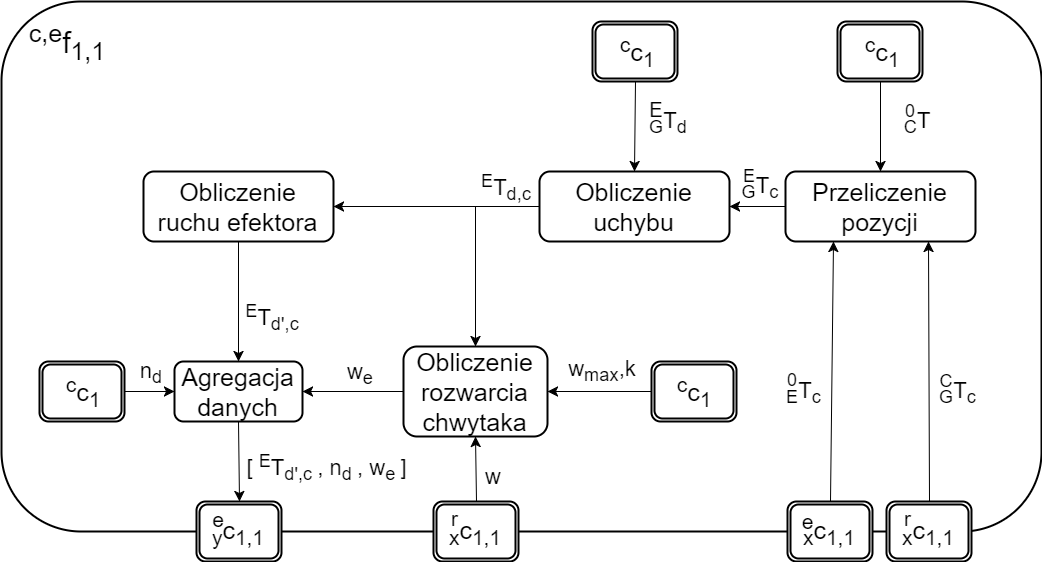
\includegraphics[width=0.9\textwidth]{PS_funkcje1v1.png}
	\caption{Funkcja przej\'scia podsystemu sterowania $^{c,e}f_{1,1}$}
	\label{fig::PS_funkcje1v1}
\end{figure}
\item Funkcja przej\'scia między podsystemem sterowania a pamięcią wewnętrzną:
\[ ^cc_{1}^{i+1}= ^{c,c}f'_{1,1}(^cc_1^i,^e_xc_{1,1}^i,^r_xc_{1,1}^i) = ^{c,c}f'_{1,1}(w_{max},k,^E_GT_d,^0_CT,^0_ET_c,^C_GT_c,w) = [STATUS,w_p]\]
\begin{figure}[H]
	\centering
	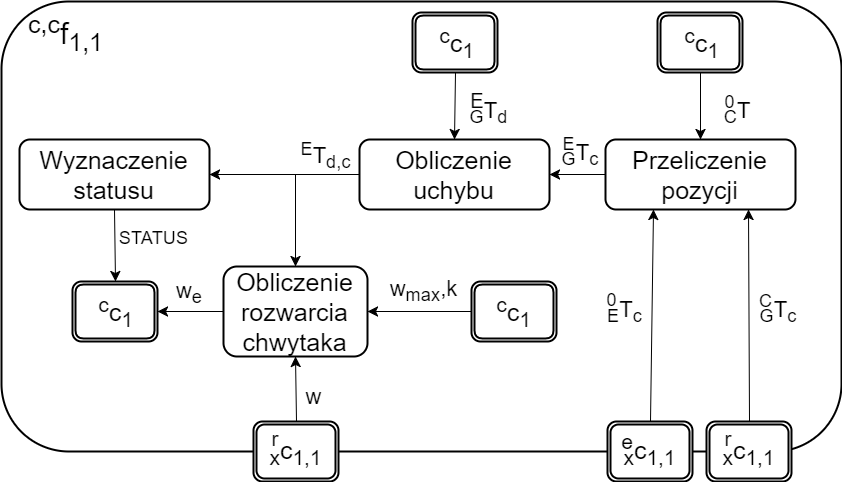
\includegraphics[width=0.9\textwidth]{PS_funkcje2v1.png}
	\caption{Funkcja przej\'scia podsystemu sterowania $^{c,c}f_{1,1}$}
	\label{fig::PS_funkcje2v1}
\end{figure}
\item Opis bloków:
\begin{itemize}
\item Przeliczenie pozycji obiektu do układu efektora: 
\[^E_GT_c = ^0_ET_c^{-1}~^0_CT~^C_GT_c\]
\item Obliczenie uchybu: 
\[^ET_{d,c}=^E_GT_c~^E_GT_d^{-1}\]
\item Obliczenie ruchu efektora:
\[^ET_{d',c}=R(^ET_{d,c})\]
\item Obliczenie rozwarcia chwytaka (w momencie osiągnięcia przez końcówkę pożądanej pozycji wględem obiektu chwytak zamyka się na szeroko\'sć równą szeroko\'sci sze\'scianu pomniejszoną o pewien margines, w przeciwnym przypadku chwytak jest rozwarty na maksymalną szeroko\'sć):
\newline
IF $^ET_{d',c}$ == 0 THEN \newline
$w_e = w-k$; \newline
ELSE \newline
$w_e = w_{max}$; \newline
ENDIF
\item Wyznaczenie statusu (w momencie osiągnięcia przez końcówkę pożądanej pozycji względem obiektu status podsystemu sterownia zmienia się na BUSY, za\'s w przeciwnym przypadku pozostaje FREE):
\newline
IF $^ET_{d',c}$ == 0 THEN \newline
$STATUS = BUSY$; \newline
ELSE \newline
$STATUS = FREE$; \newline
ENDIF
\end{itemize}
\end{itemize}

\item Funkcje przej\'scia dla zachowania \textit{``Odłóż''}:
\begin{itemize}
\item Funkcja przej\'scia między podsystemem sterowania a efektorem wirtualnym:
\[ ^e_yc_{1,1}^{i+1}= ^{c,e}f'_{1,2}(^cc_1^i,^e_xc_{1,1}^i)= ^{c,e}f'_{1,2}(n_d,w_{max},w_p,^E_PT_d,^0_PT,^0_ET_c)=[ ^ET_{d',c},n_d,w_e ]\]
\begin{figure}[H]
	\centering
	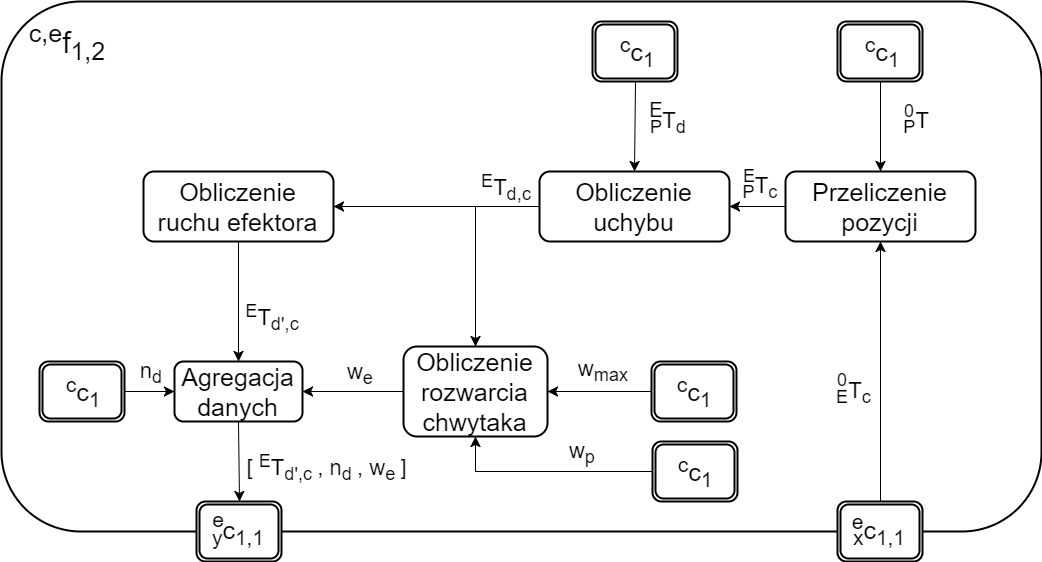
\includegraphics[width=0.83\textwidth]{PS_funkcje1v2.png}
	\caption{Funkcja przej\'scia podsystemu sterowania $^{c,e}f_{1,2}$}
	\label{fig::PS_funkcje1v2}
\end{figure}
\item Funkcja przej\'scia między podsystemem sterowania a pamięcią wewnętrzną:
\[ ^cc_{1}^{i+1}= ^{c,c}f'_{1,2}(^cc_1^i,^e_xc_{1,1}^i)= ^{c,c}f'_{1,2}(w_{max},w_p,^E_PT_d,^0_PT,^0_ET_c) = [STATUS,w_p]\]
\begin{figure}[H]
	\centering
	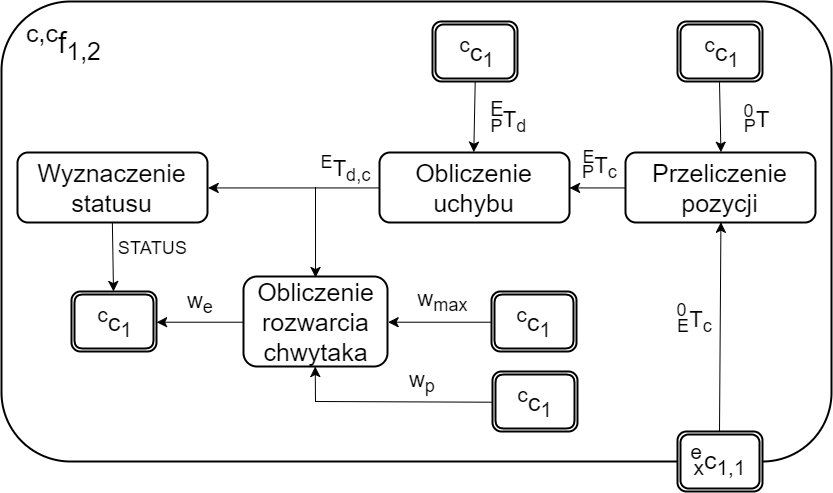
\includegraphics[width=0.83\textwidth]{PS_funkcje2v2.png}
	\caption{Funkcja przej\'scia podsystemu sterowania $^{c,c}f_{1,2}$}
	\label{fig::PS_funkcje2v2}
\end{figure}
\item Opis bloków:
\begin{itemize}
\item Przeliczenie pozycji pojemnika do układu efektora: 
\[^E_PT_c = ^0_ET_c^{-1}~^0_PT\]
\item Obliczenie uchybu: 
\[^ET_{d,c}=^E_PT_c~^E_PT_d^{-1}\]
Obliczenie ruchu efektora:
\[^ET_{d',c}=R(^ET_{d,c})\]
\item Obliczenie rozwarcia chwytaka (w momencie osiągnięcia przez końcówkę pożądanej pozycji względem pojemnika chwytak rozwiera się szeroko\'sć maksymalną, za\'s w przeciwnym przypadku chwytak pozostaje zwarty na taką samą szeroko\'sć co w poprzednim kroku):
\newline
IF $^ET_{d',c}$ == 0 THEN \newline
$w_e = w_{max}$; \newline
ELSE \newline
$w_e = w_p$; \newline
ENDIF
\item Wyznaczenie statusu (w momencie osiągnięcia przez końcówkę pożądanej pozycji względem pojemnika status podsystemu sterownia zmienia się na FREE, za\'s w przeciwnym przypadku pozostaje BUSY):
\newline
IF $^ET_{d',c}$ == 0 THEN \newline
$STATUS = FREE$; \newline
ELSE \newline
$STATUS= BUSY$; \newline
ENDIF
\end{itemize}
\end{itemize}

\end{itemize}


%%%%%%%%%%%%%%%%%%%%%%%%%%%%%%%%%%%%%%%%%%%%%%%%%%%%%%%%%%%%%%%%%%%%%%%%%%%

\subsection{Wirtualny efektor}

\begin{figure}[H]
	\centering
	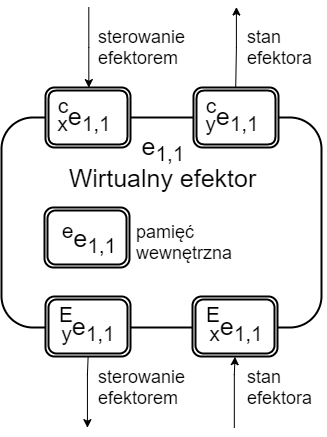
\includegraphics[width=0.38\textwidth]{wirtualny_efektor.png}
	\caption{Wirtualny efektor}
	\label{fig::wirtualny_efektor}
\end{figure}

\subsubsection{Zawarto\'sć pamięci wewnętrznej oraz buforów wej\'sciowych i wyj\'sciowych}
\begin{enumerate}
\item Pamięć wewnętrzna wirtualnego efektora:
\begin{itemize}
\item  $^ee_{1,1}$ [$\Theta_p, w_p$] - poprzednie położenie stawów (wykorzystywane przy rozwiązywaniu odwrotnego zadania kinemtyki), poprzednie rozwarcie chwytaka.
\end{itemize}
\item Bufor wej\'sciowy od podsystemu sterowania:
\begin{itemize}
\item  $^c_xe_{1,1}$ [$^ET_{d',c}, n_d, w_e$] - względna kartezjańska pozycja pożądana oraz liczba kroków zachowania, rozwarcie chwytaka.
\end{itemize}
\item Bufor wyj\'sciowy do podsystemu sterowania:
\begin{itemize}
\item $^c_ye_{1,1}$ [$^0_ET_c$] - aktualna kartezjańska pozycja bezwzględna.
\end{itemize}
\item Bufory wej\'sciowy od rzeczywistego efektora:
\begin{itemize}
\item $^E_xe_{1,1}$ [$m_c$] - aktualne położenie wałów silników.
\end{itemize}
\item Bufory wyj\'sciowy do rzeczywistego efektora:
\begin{itemize}
\item $^E_ye_{1,1}$ [$m_{d'}, w_e$] - pożądany przyrost położenia wałów silników, rozwarcie chwytaka.
\end{itemize}
\end{enumerate}

%------------------------------------------------------------------------------------------------------------------------------------------------------------------------------------------------------------

\subsubsection{Automat skończony, zachowania, warunki początkowe i końcowe}
\begin{figure}[H]
	\centering
	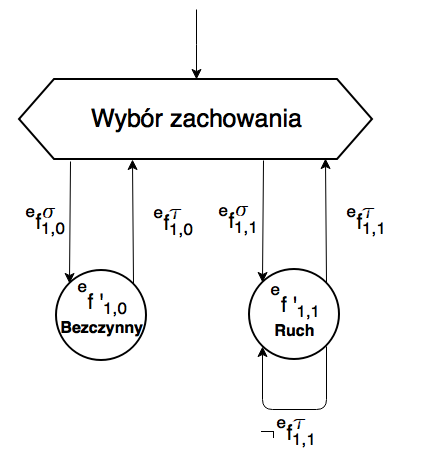
\includegraphics[width=0.55\textwidth]{WE_automat.png}
	\caption{Automat skończony zachowań wirtualnego efektora}
	\label{fig::WE_automat}
\end{figure}

Wirtualny efektor ma okre\'slone dwa zachowania: \textit{``Bezczynny''} oraz \textit{``Ruch''}. 
\newline
\begin{itemize}
\item Warunki początkowe i końcowe dla zachowania \textit{``Bezczynny''}:
\[^e_+B_{1,0}( ^{e}f'_{1,0}, ^ef^\tau_{1,0} )\]
\[^ef^\tau_{1,0} \triangleq \mbox{True}\]
\[^ef^\sigma_{1,0} \triangleq \neg \mbox{new}([^ET_{d',c}, n_d, w_e])= \neg \mbox{new}([^c_xe_{1,1}])\]
Generator następnego stanu wirtualnego efektora:
\[ _ye^{i+1}_{1,1} = ^{e}f'_{1,0}(_xe^i_{1,1})\]

\item Warunki początkowe i końcowe dla zachowania \textit{``Ruch''}:
\[^e_+B_{1,1}( ^{e}f'_{1,1}, ^ef^\tau_{1,1} )\]
\[^ef^\tau_{1,1} \triangleq \mbox{osiągnięto założoną liczbę kroków} ~n_d\]
\[^ef^\sigma_{1,1} \triangleq \mbox{new}([^ET_{d',c}, n_d, w_e]) = \mbox{new}([^c_xe_{1,1}]) = \neg ^ef^\sigma_{1,0}\]
Generator następnego stanu wirtualnego efektora:
\[ _ye^{i+1}_{1,1} = ^{e}f'_{1,1}(_xe^i_{1,1})\]
\end{itemize}

Wielko\'sć $n_d$ okre\'sla liczbę kroków zachowania, która jest równa ilorazowi kroku dyskretyzacji podsystemu sterowania i kroku dyskretyzacji wirtualnego efektora. W jego wyniku, każda funkcja przej\'scia jest wykonywana $n_d$ razy w wyniku czego za każdym razem uaktualniane są bufory do kontaktu z rzeczywistym manipulatorem i pamięć wewnętrzna. Co $n_d$ kroków uaktualniane są bufory do kontaktu z podsystemem sterowania.

%------------------------------------------------------------------------------------------------------------------------------------------------------------------------------------------------------------

\subsubsection{Funkcje przej\'scia}

\begin{itemize}
\item Funkcje przej\'scia dla zachowania \textit{``Ruch''}:
\begin{itemize}
\item Funkcja przej\'scia między efektorem wirtualnym a efektorem rzeczywistym:
\[^E_ye^{i+1}_{1,1}=^{e,E}f'_{1,1}(^c_xe_{1,1}^{i},^ee_{1,1}^{i},^E_xe_{1,1}^{i})=^{e,E}f'_{1,1}(w_e,^ET_{d',c},\Theta_p,m_c)=[m_{d'},w_e] \]
\begin{figure}[H]
	\centering
	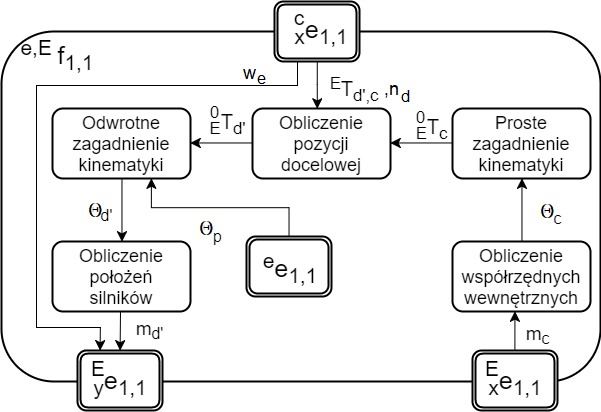
\includegraphics[width=0.75\textwidth]{WE_funkcje1.png}
	\caption{Funkcja przej\'scia wirtualnego efektora $^{e,E}f_{1,1}$}
	\label{fig::WE_funkcje1}
\end{figure}
\item Funkcja przej\'scia między efektorem wirtualnym a podsystemem sterowania:
\[^c_ye^{i+1}_{1,1}=^{e,c}f'_{1,1}(^E_xe_{1,1}^{i})=^{e,c}f'_{1,1}(m_c)=^0_ET_c \]
\begin{figure}[H]
	\centering
	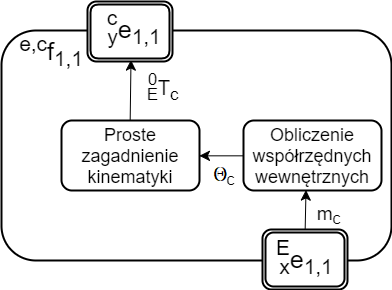
\includegraphics[width=0.45\textwidth]{WE_funkcje2.png}
	\caption{Funkcja przej\'scia wirtualnego efektora $^{e,c}f_{1,1}$}
	\label{fig::WE_funkcje2}
\end{figure}
\item Funkcja przej\'scia między efektorem wirtualnym a pamięcią wewnętrzną(zapis do pamięci aktualnego położenia stawów i rozwarcia chwytaka):
\[^ee^{i+1}_{1,1}=^{e,e}f'_{1,1}(^c_xe_{1,1}^i,^E_xe_{1,1}^{i})=^{e,c}f'_{1,1}(w_e,m_c)= [ \Theta_c, w_e ] \]
\begin{figure}[H]
	\centering
	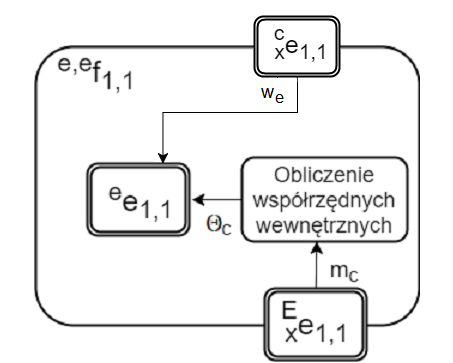
\includegraphics[width=0.45\textwidth]{WE_funkcje3.png}
	\caption{Funkcja przej\'scia wirtualnego efektora $^{e,e}f_{1,1}$}
	\label{fig::WE_funkcje3}
\end{figure}
\end{itemize}
\item Funkcje przej\'scia dla zachowania \textit{``Bezczynny''}:
\begin{itemize}
\item Funkcja przej\'scia między efektorem wirtualnym a efektorem rzeczywistym ( efektor rzeczywisty nie wykonuje ruchu, rozwarcie chwytaka pozostaje bez zmian-wczytanie z pamięci wewnętrznej ):
\[^{e,E}f'_{1,0}\triangleq^E_ye^{i+1}_{1,1}=
\begin{cases}
m_{d'} = 0 \\
w_e = w_p
\end{cases} \]
\item Funkcja przej\'scia między efektorem wirtualnym a podsystemem sterowania:
\[^c_ye^{i+1}_{1,1}=^{e,c}f'_{1,0}(^ee_{1,1}^{i})=^{e,c}f'_{1,0}(\Theta_p)=^0_ET_c \]
\begin{figure}[H]
	\centering
	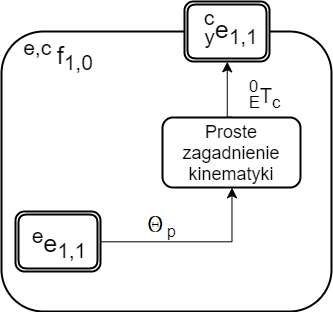
\includegraphics[width=0.45\textwidth]{WE_funkcje2v2.png}
	\caption{Funkcja przej\'scia wirtualnego efektora $^{e,c}f_{1,0}$}
	\label{fig::WE_funkcje2v2}
\end{figure}
\item Funkcja przej\'scia między efektorem wirtualnym a pamięcią wewnętrzną ( nie występuje zapis nowych danych do bufora pamięci wewnętrznej efektora wirtualnego ):
\[^ee^{i+1}_{1,1}=^{e,e}f'_{1,0}(^ee_{1,1}^{i})=^{e,e}f'_{1,0}(\Theta_p,w_p)=^ee_{1,1}^{i}=[ \Theta_p, w_p ] \]
\end{itemize}
\end{itemize}

%%%%%%%%%%%%%%%%%%%%%%%%%%%%%%%%%%%%%%%%%%%%%%%%%%%%%%%%%%%%%%%%%%%%%%%%%%%

\subsection{Wirtualny receptor}
\begin{figure}[H]
	\centering
	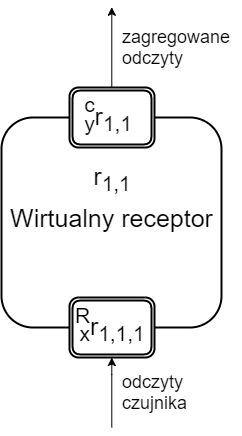
\includegraphics[width=0.27\textwidth]{wirtualny_receptor.png}
	\caption{Wirtualny receptor}
	\label{fig::wirtualny_receptor}
\end{figure}

\subsubsection{Zawarto\'sć pamięci wewnętrznej oraz buforów wej\'sciowych i wyj\'sciowych}

\begin{enumerate}
\item Bufor wej\'sciowy od rzeczywistego receptora:
\begin{itemize}
\item $^R_xr_{1,1,1}$ [$^CI_{RGB}$] - obraz otrzymywany z kamery.
\end{itemize}
\item Bufor wyj\'sciowy do podsystemu sterowania:
\begin{itemize}
\item $^c_yr_{1,1}$ [$^C_GT_c, w$] - aktualna pozycja rozpoznawanego obiektu(czerwonego sze\'scianu) względem kamery, szeroko\'sć obiektu.
\end{itemize}
\end{enumerate}

%------------------------------------------------------------------------------------------------------------------------------------------------------------------------------------------------------------

\subsubsection{Automat skończony, zachowania, warunki początkowe i końcowe}
\begin{figure}[H]
	\centering
	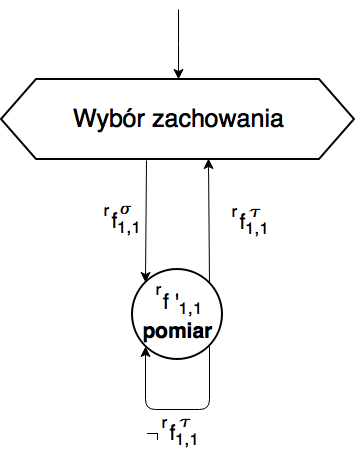
\includegraphics[width=0.45\textwidth]{WR_automat.png}
	\caption{Jednostanowy automat skończony zachowań wirtualnego receptora}
	\label{fig::WR_automat}
\end{figure}

Dla wirtualnego receptora okre\'slono jedno zachowanie - \textit{``Pomiar''}. Jedno zachowanie implikuje jednostanowy automat skończony. Założono, że jet to zachowanie nieskończone(bez wyzwalania), zatem warunek końcowy $^rf^\tau_{1,1}$ jest zawsze \textit{False}, za\'s początkowy  $^rf^\sigma_{1,1}$ jest zawsze \textit{True}.
\newline
Warunki początkowe i końcowe dla zachowania \textit{``Pomiar''}:
\[^r_+B_{1,1}( ^{r}f'_{1,1}, ^rf^\tau_{1,1} )\]
\[^rf^\tau_{1,1} \triangleq \mbox{False}\]
\[^rf^\sigma_{1,1} \triangleq \mbox{True}\]
Generator następnego stanu wirtualnego receptora:
\[ _yr^{i+1}_{1,1} = ^{r}f'_{1,1}(_xr^i_{1,1})\]

%------------------------------------------------------------------------------------------------------------------------------------------------------------------------------------------------------------

\subsubsection{Funkcje przej\'scia}
Funkcja przej\'scia między receptorem wirtualnym a podsystemem sterowania:
\[ _y^cr^{i+1}_{1,1} = ^{r,c}f'_{1,1}(_x^Rr_{1,1,1}^i)=^{r,c}f'_{1,1}(^CI_{RGB})=[^C_GT_c,w]\]
\begin{figure}[H]
	\centering
	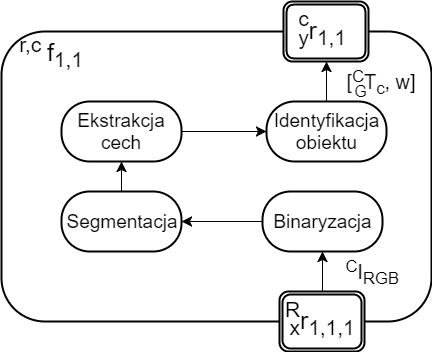
\includegraphics[width=0.45\textwidth]{WR_funkcje.png}
	\caption{Funkcja przej\'scia wirtualnego receptora $^{r,c}f_{1,1}$}
	\label{fig::WR_funkcje}
\end{figure}
Funkcja przej\'scia powoduje zagregowanie informacji otrzymywanych z rzeczywistego receptora. Obraz otrzymywany z kamery (bufor $_x^Rr_{1,1,1}$) podlegla operacjom w wyniku czego otrzymuje się położenie obiektu względem kamery oraz jego szeroko\'sć.

%%%%%%%%%%%%%%%%%%%%%%%%%%%%%%%%%%%%%%%%%%%%%%%%%%%%%%%%%%%%%%%%%%%%%%%%%%%

\subsection{Kroki dyskretyzacji}

Typowe kamery RGB charkteryzują się szybko\'scią wy\'swietlania obrazów na poziomie 25 \textit{fps}, co daje jedną klatkę co 40 ms. Dla maskymalnej prędko\'sci ta\'smociągu równej 0.1m/s przyjęcie takiego kroku dyskretyzacji wprowadza maksymalną zmianę położenia obiektu równą 4 mm, co jest warto\'scią akceptowalną. Zatem dobrano krok dyskretyzacji czasu wirtualnego receptora równy 40 ms. Mniejsza warto\'sć kroku dyskretyzacji nie przyniosłaby dodatkowej korzy\'sci, gdyż kolejne klatki obrazu z kamery pojawiałyby się niezmiennie co 40 ms (zatem nie następowałoby dostarczane nowych informacji pomiędzy kolejnymi chwilami próbkowania). Wykorzystując powszechny protokół komunikacji EtherNet/IP o szybko\'sci transmisji do 100Mbit/s opóźnienie transmisyjne, przy przesyłaniu klatek obrazu z kamery, można pominąć.
\newline
Dla wirtualnego efektora dobrano warto\'sć kroku dyskretyzacji typowy dla sterowników robotów równy 1 ms. Uwzględniając maksymalną prędko\'sć liniową końcówki manipulatora równą 1 m/s, można obliczyć maksymalną odległo\'sć o jaką przemie\'sci się końcówka równą 1 mm. Jest to warto\'sć, która pozwala na płynne oraz szybkie przemieszczanie końcówki manipulatora. Ze względu na niewielką ilo\'sć przesyłanych danych opóźnienia transmisyjne można pominąć.
\newline
Ze względu na znaczą dokładno\'sć manipulatorów oraz większą prędko\'sć końcówki manipulatora względem prędko\'sci ta\'smociągu przyjęto okres próbkowania podsystemu sterowania równy 10 ms. W związku z tym wirtualny efektor wykonuje dziesięć kroków podczas jednego kroku podsystemu sterownia. Zatem co 1 cm jest wprowadzana korekta ustawienia końcówki względem punktu docelowego. Warto\'sć ta jest odpowienia biorąć pod uwagę maksymalną odległo\'sć jaką może przebyć obiekt na ta\'smociągu.

\end{document}